\documentclass[a4paper,runningheads]{llncs}

\usepackage[utf8]{inputenc}
\usepackage[T1]{fontenc}
\usepackage{lmodern}
\usepackage[english]{babel}
\usepackage{hyperref}
\usepackage{comment}
\usepackage{boxedminipage}
\usepackage{graphicx}
\usepackage{booktabs}
\usepackage{wrapfig}
\usepackage{listings}
\usepackage{xcolor}
\usepackage{rotating}
\usepackage{xstring}

\newcommand{\ooo}[1]{\textsf{101#1}}
\newcommand{\oneohone}{\ooo{}}
\newcommand{\MediaWiki}{\textsf{MediaWiki}}
\newcommand{\Wikipedia}{\textsf{Wikipedia}}
\newcommand{\WikipediaUrl}{http://en.wikipedia.org/wiki}
\newcommand{\WikipediaPage}[1]{%
  \protect\StrSubstitute{#1}{ }{_}[\wikiurl]%
  \protect\href{\WikipediaUrl/\wikiurl}{\emph{#1}}}
\newcommand{\WikipediaCategory}[1]{%
  \protect\StrSubstitute{Category:#1}{ }{_}[\wikiurl]%
  \protect\href{\WikipediaUrl/\wikiurl}{\emph{#1}}}
\newcommand{\WikiTaxEmptyCell}{--}
\newcommand{\WikiTax}{\textsf{WikiTax}}
\newcommand{\WikiTaxCategory}[1]{\WikipediaCategory{#1}}
\newcommand{\WikiTaxSubcategory}[1]{\WikipediaCategory{#1}}
\newcommand{\WikiTaxComment}[1]{#1}
\newcommand{\WikiTaxNewLine}{\\\hline}

%\clubpenalty = 10000 
%\widowpenalty = 10000 
%\displaywidowpenalty = 10000

\colorlet{punct}{red!60!black}
\definecolor{background}{HTML}{EEEEEE}
\definecolor{delim}{RGB}{20,105,176}
\colorlet{numb}{magenta!60!black}

\lstdefinelanguage{json}{
    basicstyle=\normalfont\ttfamily\scriptsize,
    showstringspaces=false,
    breaklines=true,
    frame=lines,
    backgroundcolor=\color{background},
    literate=
     *{0}{{{\color{numb}0}}}{1}
      {1}{{{\color{numb}1}}}{1}
      {2}{{{\color{numb}2}}}{1}
      {3}{{{\color{numb}3}}}{1}
      {4}{{{\color{numb}4}}}{1}
      {5}{{{\color{numb}5}}}{1}
      {6}{{{\color{numb}6}}}{1}
      {7}{{{\color{numb}7}}}{1}
      {8}{{{\color{numb}8}}}{1}
      {9}{{{\color{numb}9}}}{1}
      {:}{{{\color{punct}{:}}}}{1}
      {,}{{{\color{punct}{,}}}}{1}
      {\{}{{{\color{delim}{\{}}}}{1}
      {\}}{{{\color{delim}{\}}}}}{1}
      {[}{{{\color{delim}{[}}}}{1}
      {]}{{{\color{delim}{]}}}}{1},
}

\author{Ralf L\"ammel \and Dominik Mosen \and Andrei Varanovich}
\institute{University of Koblenz-Landau, Software Languages Team}
%\title{Exploration of \Wikipedia's categories for software languages with \WikiTax}
\title{Method and tool support for classifying software languages with \Wikipedia}
%\subtitle{Tool demonstration}

\begin{document}

\maketitle

\begin{abstract} 

  \Wikipedia{} provides useful input for efforts on mining taxonomies
  or ontologies in specific domains. In particular, \Wikipedia's
  categories serve classification. In this paper, we describe a
  method and a corresponding tool, \WikiTax, for exploring
  \Wikipedia's category graph with the objective of supporting the
  development of a classification of software languages. The category
  graph is extracted level by level. The extracted graph is visualized
  in a tree-like manner. Category attributes (i.e., metrics) such as
  depth are visualized. Irrelevant edges and nodes may be
  excluded. These exclusions are documented while using a manageable
  and well-defined set of `exclusion types' as comments.
\end{abstract}

%%%%%%%%%%%%%%%%%%%%%%%%%%%%%%%%%%%%%%%%%%%%%%%%%%%%%%%%%%%%

%%%%%%%%%%%%%%%%%%%%%%%%%%%%%%%%%%%%%%%%%%%%%%%%%%%%%%%%%%%%

\section{Introduction}
\label{S:intro}

\vspace{-27\in}

Ever since 2008, the calls for papers for the \emph{Software Language Engineering} (SLE) conference\footnote{\url{http://planet-sl.org/}} have contained slightly different, more implicit or more explicit definitions of the term `software language'. Other community material contains yet other definition attempts; see, for example, the IEEE TSE special section on SLE in 2009~\cite{FavreGLW09}. At SLEBOK 2012 (i.e., an SLE 2012 satellite event dedicated to the the SL(E) body of knowledge), the attendees were also getting into the issue of what exactly a software language is.

A \emph{classification} of software languages is a useful (if not necessary) pillar of a definition of `software language'. Such classification is the topic of the present paper. One branch of software languages appears to be well understood. That is, \emph{programming languages} are obviously \emph{software languages} and they may be classified in terms of criteria and concepts as organized, for example, in textbooks on programming languages, programming paradigms, and programming language theory such as~\cite{Mosses92,Sebesta12}. There is also scholarly (dated) work on the classification of programming languages~\cite{BabenkoRY75,DoyleS87}. Actually quite a few sets of criteria or concepts exist for programming languages; there is no obvious contender; there is no comprehensive classification. Several classes of languages (other than programming languages) have been classified in scholarly work, e.g., model transformation languages~\cite{CzarneckiH06}, business rule modeling languages~\cite{SkalnaG12}, visual languages~\cite{BottoniG04,BurnettB94,MarriottM97}, and architecture description languages~\cite{MedvidovicT00}. The ultimate taxonomy of software languages should subsume and integrate existing, fragmented classifications in a transparent manner. The \emph{101companies} project\footnote{\url{http://101companies.org/}} hosts efforts targeted at such a taxonomy, but the results are of limited use and quality so far. 

In this paper, we try to inform the apparent classification challenge for software languages by means of exploring \Wikipedia. Obviously, \Wikipedia{} contains substantial amounts of taxonomy-like (if not ontology-like) information---also for software languages (without though embracing the actual term, at the time of writing). For instance, there are hierarchically organized categories such as \WikipediaCategory{Computer languages}, \WikipediaCategory{Programming languages}, and \WikipediaCategory{Programming language classification} that seem to apply; yet other categories may be relevant. Accordingly, we describe a method and a corresponding tool, \WikiTax, for exploring \Wikipedia's category graph. Exploration is supported in a manner such that a domain expert can reduce the category graph so that a classification emerges. The overall approach is not specific to software languages, but we apply it to software languages throughout the paper. 

\vspace{-27\in}

\paragraph*{\textbf{Contribution}} We do not claim to have converged on a good candidate taxonomy for software languages. Rather we contribute procedural, tool-supported elements of a method towards development of the ultimate taxonomy. The resulting tool, \WikiTax, is a rather simple graph exploration tool, which however includes a few domain-specific features not available in more generic functionality for searching and exploring \Wikipedia's category graph.

\vspace{-27\in}

\paragraph*{\textbf{Road-map}} \S\ref{S:approach} describes the overall exploration approach and sketches corresponding tool support as implemented by \WikiTax. \S\ref{S:study} explores \Wikipedia{} categories related to software languages. \S\ref{S:concl} concludes the paper. The source code of \WikiTax, a comprehensive manual, and all data covered in this paper are available online.\footnote{\url{https://github.com/dmosen/wiki-analysis}}

%%%%%%%%%%%%%%%%%%%%%%%%%%%%%%%%%%%%%%%%%%%%%%%%%%%%%%%%%%%%

%%%%%%%%%%%%%%%%%%%%%%%%%%%%%%%%%%%%%%%%%%%%%%%%%%%%%%%%%%%%

\section{Exploring \Wikipedia{} with \WikiTax} 
\label{S:approach}

%%%%%%%%%%%%%%%%%%%%%%%%%%%%%%%%%%%%%%%%%%%%%%%%%%%%%%%%%%%%

\vspace{-27\in}

\paragraph*{\textbf{\Wikipedia's category graph}}

\Wikipedia{} uses several means of organizing its information: plain
links giving rise to an article graph, designated article lists,
portals meant to introduce users to key topics, info-boxes for
semantic (`typed') data, and categories giving rise to a category
graph for the classification of articles. When it comes to taxonomy
mining, the category graph is particularly relevant; the graph is
accessible, for example, through the \MediaWiki{} API, which is the
access path chosen by \WikiTax.

% \footnote{\url{http://www.mediawiki.org/wiki/API:Main_page}}

%%%%%%%%%%%%%%%%%%%%%%%%%%%%%%%%%%%%%%%%%%%%%%%%%%%%%%%%%%%%

\vspace{-27\in}

\paragraph*{\textbf{Graph extraction}}

Initially, \WikiTax{} is pointed to a root category (level 0) for
extraction. Iteratively, subcategories and pages (in fact, page
titles) can be extracted level by level or exhaustively. Exhaustive
extraction may take minutes to hours depending on the root
category. The \Wikipedia{} category graph contains many surprising
edges, which would easily imply inclusion of large, arguably
irrelevant subgraphs. Thus, extraction is controllable.

%%%%%%%%%%%%%%%%%%%%%%%%%%%%%%%%%%%%%%%%%%%%%%%%%%%%%%%%%%%%

\vspace{-27\in}

\paragraph*{\textbf{Graph reduction}}

\WikiTax{} supports reduction of the graph---both during
(level-by-level) extraction and post extraction. Reduction boils down
to the exclusion of nodes, i.e., categories. (In fact, we may also
remove individual edges, given that a category may have multiple
parent categories.)  A category would be removed, if domain knowledge
suggests that the category at hand does not serve the intended kind of
classification, e.g., classification of software languages in our
case. When exclusion is performed during extraction, then the excluded
nodes (edges) are ignored during subsequent extraction steps. When
exclusion is performed post extraction, then nodes (edges) are only
blacklisted, without actually reducing the graph. In this manner,
exclusion decisions can be revisited.

%%%%%%%%%%%%%%%%%%%%%%%%%%%%%%%%%%%%%%%%%%%%%%%%%%%%%%%%%%%%

\begin{figure}[t!]
\begin{center}
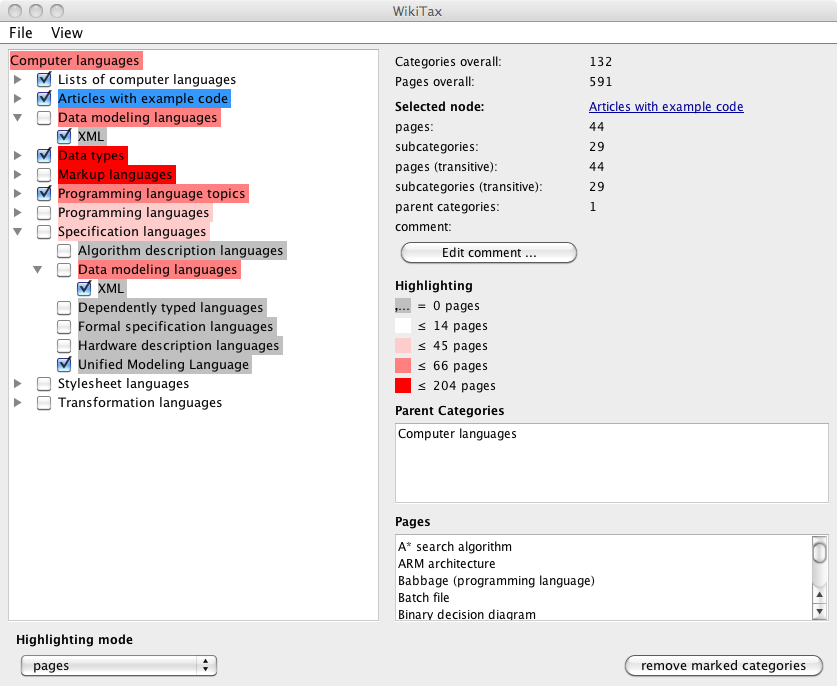
\includegraphics[width=.98\textwidth]{figures/clLevel12.png}
\end{center}
\vspace{-66\in}
\caption{Exploration of level 1 and 2 subcategories of \emph{Computer languages}.}
\label{F:clLevel12}
\vspace{-42\in}
\end{figure}

%%%%%%%%%%%%%%%%%%%%%%%%%%%%%%%%%%%%%%%%%%%%%%%%%%%%%%%%%%%%

\vspace{-27\in}

\paragraph*{\textbf{\WikiTax's visualization}}

\autoref{F:clLevel12} shows the \WikiTax{} exploration view after the
extraction of levels 1 and 2 starting from the category
\WikipediaCategory{Computer languages}. Some edges are marked for
exclusion. (Exclusion would be confirmed with the `removal'
button.)  The marked categories are to be excluded because domain
knowledge suggests that these categories do not serve language
classification in a conceptual manner. Highlighting is
applied to the categories according to the metric of immediate member
pages. In the figure, the category \WikipediaCategory{Articles with
  example code} is selected so that extra data is shown in the panel
on the right, e.g., member pages. All categories and pages are
clickable to navigate to \Wikipedia.

%%%%%%%%%%%%%%%%%%%%%%%%%%%%%%%%%%%%%%%%%%%%%%%%%%%%%%%%%%%%

\begin{figure}[ht]
\centering
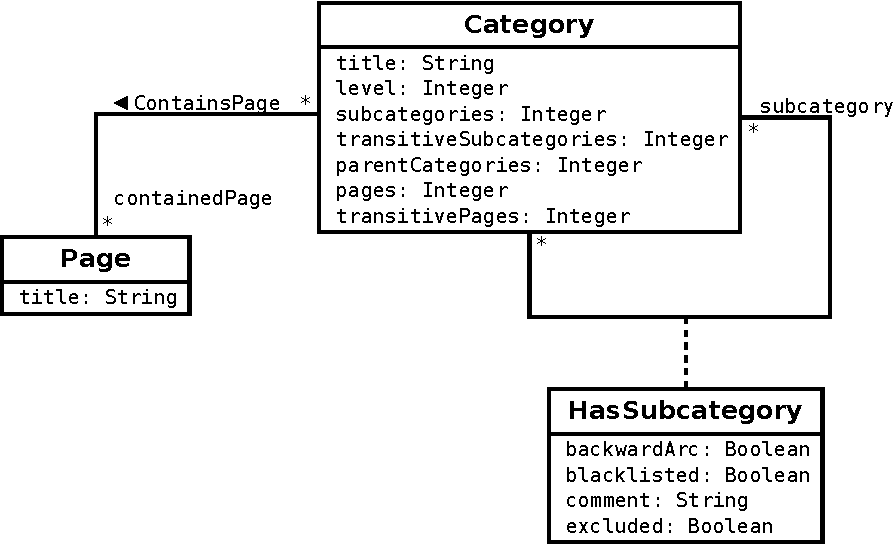
\includegraphics[width=0.75\textwidth]{figures/full_schema.pdf} 
\caption{Metamodel of the \WikiTax{} category graph.}
\label{F:metamodel}
\vspace{-42\in}
\end{figure}

%%%%%%%%%%%%%%%%%%%%%%%%%%%%%%%%%%%%%%%%%%%%%%%%%%%%%%%%%%%%

\vspace{-27\in}

\paragraph*{\textbf{\WikiTax's metamodel}}

\WikiTax{} operates on an enhanced category graph; see the metamodel
in \autoref{F:metamodel}. Thus, each category associates with contained pages and
subcategories. The subcategory associations are attributed to keep
track of metadata as follows:

\vspace{-27\in}

{\small

\begin{description}
\item[\ \ backwardArc] Marker for cyclic edges in the category graph.
\item[\ \ blacklisted] Marker for categories blacklisted past extraction.
\item[\ \ excluded] Marker for categories excluded during reduction.
\item[\ \ comment] Label (`reason for exclusion') to be associated with the edge.
\end{description}

}

\noindent
Categories are associated with measures as follows:

\vspace{-27\in}

{\small

\begin{description}
\item[\ \ level] The level 0, 1, 2, ... of the category in the graph with the root at level 0.
\item[\ \ subcategories] The number of immediate subcategories.
\item[\ \ transitiveSubcategories] The number of all subcategories.
\item[\ \ pages] The number of immediately contained pages.
\item[\ \ transitivePages] The number of all pages in this category.
\end{description}

}

\noindent
The implementation of \WikiTax{} uses the Java-based JGraLab
library\footnote{\url{https://github.com/jgralab}} for the
  representation of (annotated) graphs with JSON as an export format.

%%%%%%%%%%%%%%%%%%%%%%%%%%%%%%%%%%%%%%%%%%%%%%%%%%%%%%%%%%%%

\vspace{-27\in}

\paragraph*{\textbf{Exclusion types}} A methodologically important
aspect of graph reduction is that reasons for category exclusion are
not just simply documented by a comment, but a manageable,
well-defined set of exclusion types is to be developed over time. For
instance, the category \WikipediaCategory{Unified Modeling Language}
could be said to be of an exclusion type `Singleton classifier' to
mean that this category, by design, is primarily concerned with a
single language, i.e., UML in this case; the other members or
subcategories of the category are concerned with UML concepts, tools,
and other related artifacts. \S\ref{S:study} lists several more
exclusion types. The aggregation and use of exclusion types captures
domain knowledge and insight into \Wikipedia's category graph in a
transparent manner.

%%%%%%%%%%%%%%%%%%%%%%%%%%%%%%%%%%%%%%%%%%%%%%%%%%%%%%%%%%%%

%%%%%%%%%%%%%%%%%%%%%%%%%%%%%%%%%%%%%%%%%%%%%%%%%%%%%%%%%%%%

\section{Explorative study}
\label{S:study}

\vspace{-27\in}

In this study, we examine some \Wikipedia{} categories with two objectives: a) to retrieve some candidate classifiers of an emerging taxonomy of software languages; b) to get some experience with \Wikipedia's approach to classification and related issues of style and consistency.\footnote{All \Wikipedia{} data for this study and this paper was retrieved 7-18 June 2013.}

%%%%%%%%%%%%%%%%%%%%%%%%%%%%%%%%%%%%%%%%%%%%%%%%%%%%%%%%%%%%

\vspace{-27\in}

\paragraph*{\textbf{Designation of a root}}

\Wikipedia's classification hierarchies are complex and thus, it is not straightforward to determine a root for exploration unambiguously. However, we have established by an ad-hoc search that the category \WikipediaCategory{Computer languages} may be a suitable root: its intended coverage may be similar to what the SL(E) community has in mind for the notion of software languages.

\autoref{F:clLevel12} showed all the immediate (i.e., level 1) subcategories of the category \WikipediaCategory{Computer languages}. Several of these immediate subcategories are excluded because they are not directly concerned with the \emph{classification} of languages: \WikipediaCategory{Lists of computer languages}, \WikipediaCategory{Articles with example code}, \WikipediaCategory{Data types}, and \WikipediaCategory{Programming language topics}. One of the remaining immediate subcategories is the category \WikipediaCategory{Programming languages}. We found another major classifier for programming languages, namely \WikipediaCategory{Programming language classification}, which is reachable through the excluded category \WikipediaCategory{Programming language topics}.

%%%%%%%%%%%%%%%%%%%%%%%%%%%%%%%%%%%%%%%%%%%%%%%%%%%%%%%%%%%%

\begin{figure}[t!]
\begin{center}
{\small
\scalebox{0.9}{\mbox{
\begin{tabular}{l|p{3.3in}}
\textbf{Category} & \textbf{Subcategories} \\\hline
\input{data/Computer_languages.tex-twolevels}
\end{tabular}}}}
\end{center}
\vspace{-42\in}
\caption{Reduced subcategory lists for subcategories of \emph{Computer languages}.}
\label{F:twolevels}
\vspace{-42\in}
\end{figure}

%%%%%%%%%%%%%%%%%%%%%%%%%%%%%%%%%%%%%%%%%%%%%%%%%%%%%%%%%%%%

\vspace{-27\in}

\paragraph*{\textbf{Level-by-level extraction}}

We decided to extract another level to obtain a graph of manageable size. Again, we excluded several categories, if they did not meet our objective of language classification. As a result, we obtained the categories shown in \autoref{F:twolevels}. This is a pretty manageable set of language classifiers. 
It happens that they all end on ``... languages'' except for two subcategories of \WikipediaCategory{Markup languages} which end on ``... formats''. In contrast, most of the excluded categories (see below) do not end on ``... languages'' . We take this to provide a hint at the different classification styles of \Wikipedia.

%%%%%%%%%%%%%%%%%%%%%%%%%%%%%%%%%%%%%%%%%%%%%%%%%%%%%%%%%%%%

\begin{figure}[t!]
\begin{center}
{\small
\scalebox{0.88}{\mbox{
\begin{tabular}{l|l}
\textbf{Category} & \textbf{Exclusion type} \\\hline
\input{data/Computer_languages.tex-metaclassify}
\end{tabular}}}}
\end{center}
\vspace{-42\in}
\caption{Exclusion types for levels 1 and 2 of \emph{Computer languages}; this list is produced by the \WikiTax{} tool based on metadata (comments) entered by us interactively.}
\label{F:metaclassify}
\vspace{-42\in}
\end{figure}

%%%%%%%%%%%%%%%%%%%%%%%%%%%%%%%%%%%%%%%%%%%%%%%%%%%%%%%%%%%%

\vspace{-27\in}

\paragraph*{\textbf{Exclusion types}}

In order to obtain the reduced result of \autoref{F:twolevels}, we had to exclude 29 categories. This may seem like a small number, but it is clear that yet more categories must be excluded once deeper levels are explored. We used these 29 exclusions to develop a small set of exclusion types for the study; see \autoref{F:metaclassify} for the list of excluded categories with the associated exclusion type:

{\small

\begin{description}

\item[Alternative classifier] The category classifies software languages in a manner that is not related to software concepts. For instance, the category \WikipediaCategory{Academic programming languages} describes itself as being concerned with languages that are ``influential in computer science and programming language theory''.

\item[Deviating classifier] The category does not actually classify software languages. It rather classifies something else. For instance, category \WikipediaCategory{Articles with example code} describes itself as being concerned with ``articles which include reference implementations of algorithms''.

\item[Singleton classifier] The category is effectively concerned with a single software language for which it serves as a container of related entities such as technologies or standards. For instance, category \WikipediaCategory{Cascading Style Sheets} contains pages on all kinds of topics related to the CSS language.

\item[List classifier] The category collects lists or categories of lists (rather than plain categories) of software languages. For instance, category \WikipediaCategory{Lists of computer languages} has \WikipediaCategory{Lists of programming languages} as a subcategory, which in turn contains pages for some lists of languages, such as the \WikipediaPage{List of BASIC dialects}.

\item[Maintenance classifier] The category is used by the \Wikipedia{} authors to capture some information related to the maintenance of pages or categories. For instance, the category \WikipediaCategory{Uncategorized programming languages} describes itself as serving categories or pages ``which need to be classified under more specific categories''. Also: ``This category may be empty occasionally or even most of the time.''

% category \WikipediaCategory{Markup language stubs} describes itself as serving ``for stub articles relating to markup languages''. The 

\end{description}

}

%%%%%%%%%%%%%%%%%%%%%%%%%%%%%%%%%%%%%%%%%%%%%%%%%%%%%%%%%%%%

\vspace{-27\in}

\paragraph*{\textbf{An observation regarding \Wikipedia{} style}}

The resulting classification of \autoref{F:twolevels} with the remaining level-1 and level-2 subcategories is of a manageable size. We may review the classification and observe some of its characteristics in this manner. During the study, we realized, for example, an asymmetry between `query' versus `transformation'. That is, there is a category \WikipediaCategory{Transformation languages} at level 1, but there is apparently no category for `query languages', not even at level 2. Let us inspect the page for \WikipediaPage{SQL}, which is an obvious query language. It turns out that \WikipediaPage{SQL} is a member of various categories including a category \WikipediaCategory{Query languages} which in turn is a subcategory of various categories including the category \WikipediaCategory{Domain-specific programming languages} which occurred in \autoref{F:twolevels}. Let us compare this classification scheme with the one of \WikipediaPage{XSLT}, which is an obvious transformation language: it is a member of the categories \WikipediaCategory{Transformation languages}, \WikipediaCategory{Declarative programming languages}, \WikipediaCategory{Functional languages}, \WikipediaCategory{Markup languages}, \WikipediaCategory{XML-based programming languages}, and yet other categories that may count as `alternative classifiers'. However, \WikipediaPage{XSLT} (unlike \WikipediaPage{SQL}) is not a member of the category \WikipediaCategory{Domain-specific programming languages}.

\WikiTax{} is helpful in making such observations regarding consistency (or lack thereof) of classification on \Wikipedia.

%%%%%%%%%%%%%%%%%%%%%%%%%%%%%%%%%%%%%%%%%%%%%%%%%%%%%%%%%%%%

\vspace{-27\in}

\paragraph*{\textbf{Programming languages: all levels}}

According to \autoref{F:twolevels}, the subcategory of \WikipediaCategory{Computer languages} with by far the most subcategories is 
\WikipediaCategory{Programming languages}. Thus, we embarked on a more comprehensive exploration of category \WikipediaCategory{Programming languages}:

%%%%%%%%%%%%%%%%%%%%%%%%%%%%%%%%%%%%%%%%%%%%%%%%%%%%%%%%%%%%

\begin{figure}[t!]
\parbox{.48\textwidth}{
Pages

\noindent 
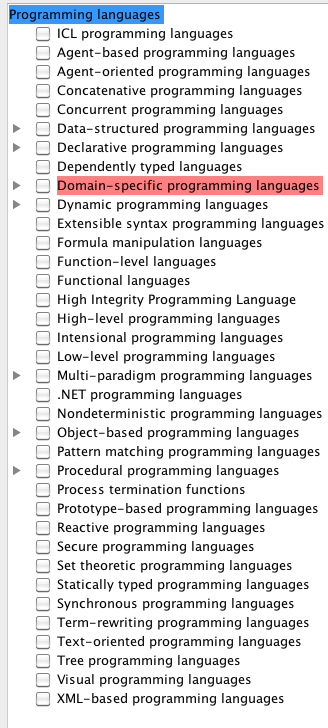
\includegraphics[width=0.45\textwidth]{figures/plPagesTransitive.png}
}\hfill\parbox{.48\textwidth}{

Categories 

\noindent 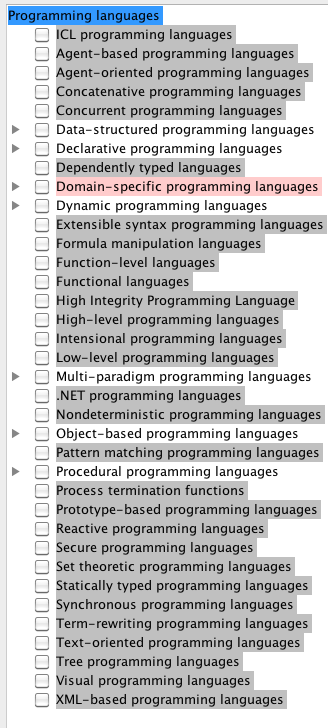
\includegraphics[width=0.45\textwidth]{figures/plSubcategoriesTransitive.png}
}

\vspace{-42\in}

\caption{Metrics-based views on \emph{Programming languages} graph.}
\label{F:plNumbers}
\vspace{-42\in}
\end{figure}

%%%%%%%%%%%%%%%%%%%%%%%%%%%%%%%%%%%%%%%%%%%%%%%%%%%%%%%%%%%%

Initially, we extracted 423 categories over 8 levels with 7515 pages. The automatic extraction took several minutes. We performed exclusion in two steps. First, we (re-) excluded those direct subcategories that already appeared in \autoref{F:metaclassify}. After such initial pruning, 288 categories with 6671 pages remained. We completed reduction at all levels of the category graph. This process required about 2 hours of manual work to determine what categories to remove and for what reason. This effort is intrinsically manual; it requires domain knowledge and involves consultation of the relevant and additional \Wikipedia{} pages. Ultimately, 79 categories over 4 levels with 1560 pages remained.  \autoref{F:plNumbers} visualizes the reduced taxonomy for two different metrics supported by \WikiTax.

On the left, the metric for the \emph{number of transitive member pages} is applied for visualization. No category is grayed out, which means that there is no category without members. Most of the categories are shown in a plain font, which means that they all carry members, but less than 25\,\% of the total members in the category \WikipediaCategory{Programming languages} (which has 1560 member pages). There is actually one heavyweight: category \WikipediaCategory{Domain-specific programming languages} carries 976 members, which is more than 50\,\% of all members; this status is expressed by 
highlighting the category.

On the right, the metric for the number of transitive subcategories is applied for visualization. Most subcategories of \WikipediaCategory{Programming languages} do not have any subcategories; thus, they are grayed out. 7 out of 36 level-1 categories carry subcategories. 6 out of these 7 categories carry only very few subcategories (less than 5). Category \WikipediaCategory{Domain-specific programming languages} carries 18 subcategories, which is more than 25\,\% of all subcategories; this status is expressed by highlighting the category.

%%%%%%%%%%%%%%%%%%%%%%%%%%%%%%%%%%%%%%%%%%%%%%%%%%%%%%%%%%%%

%%%%%%%%%%%%%%%%%%%%%%%%%%%%%%%%%%%%%%%%%%%%%%%%%%%%%%%%%%%%

\section{Conclusion}
\label{S:concl}

\vspace{-27\in}

Any domain with large data to explore (`large' in terms of what the user needs to understand) may benefit from interactive exploration possibly with editing or annotation; see tools for ontologies~\cite{BaskayaKJ10}, graphs~\cite{HaunNKTB10}, semantic data~\cite{DumasBHS12}, software bugs~\cite{HoraADBCVM12}, API usage~\cite{RooverLP13}. In this paper, we described an approach to the exploration of \Wikipedia's category graph so that candidate taxonomies can be extracted from the graph. We were specifically interested in understanding \Wikipedia's classification of software languages. To this end, we developed a domain-specific exploration tool, \WikiTax, which supports level-by-level graph extraction, metrics-based graph visualization as well as transparent and revisable graph reduction. Such designated exploration support is missing in more generic tools for searching or exploring the category graph.

The described method of graph reduction is deliberately interactive and relies on domain knowledge for transparent exclusion decisions, as opposed to any means of automated ontology extraction / generation~\cite{SuchanekKW08,WuW08}. (Without such validation, there is little hope that the resulting taxonomy would be readily meaningful.) An important conceptual contribution is our proposal to document exclusion decisions with (comments for) exclusion types, thereby making reduction more systematic and transparent. This interactive approach can be contrasted with related work on taxonomy or ontology mining, where categories are classified and additional relationships are inferred automatically, e.g., by analyzing the structure of compound category names~\cite{NastaseS08}.

We contend that the described approach provides the initial core of a method for actually developing a taxonomy for software languages (and possibly other taxonomies) on the grounds of \Wikipedia. Collaborative work and further improved tool support are needed to actually arrive at a comprehensive taxonomy. We imagine that we need powerful refactoring operations on the category graph to facilitate taxonomy extraction and enforcement of consistent style. The exploration of the category graph could also be supported by additional forms of visualization, e.g., for understanding the overlap of categories. Also, we need to generally better understand (perhaps based on an automated analysis) the different classifier styles used by \Wikipedia.

%%%%%%%%%%%%%%%%%%%%%%%%%%%%%%%%%%%%%%%%%%%%%%%%%%%%%%%%%%%%

\begin{comment}
% Another problem with Wikipedia's use of categories
\WikipediaCategory{Ada programming language} is a subcategory of, for example, \WikipediaCategory{Concurrent programming languages}, while \WikipediaPage{Ada (programming language)} is not a member page of 
\WikipediaCategory{Concurrent programming languages}, but it is a member of various other ``... programming languages'' categories. For comparison consider \WikipediaCategory{Erlang programming language}, which is also a subcategory of, for example, \WikipediaCategory{Concurrent programming languages} and \WikipediaPage{Erlang (programming language)} is also a member page of \WikipediaCategory{Concurrent programming languages}.
\end{comment}

%%%%%%%%%%%%%%%%%%%%%%%%%%%%%%%%%%%%%%%%%%%%%%%%%%%%%%%%%%%%


%%%%%%%%%%%%%%%%%%%%%%%%%%%%%%%%%%%%%%%%%%%%%%%%%%%%%%%%%%%%

\bibliographystyle{splncs03}
\bibliography{paper}

%%%%%%%%%%%%%%%%%%%%%%%%%%%%%%%%%%%%%%%%%%%%%%%%%%%%%%%%%%%%

\end{document}

%%%%%%%%%%%%%%%%%%%%%%%%%%%%%%%%%%%%%%%%%%%%%%%%%%%%%%%%%%%%
